\subsection{الگوهای معماری امنیت و قابلیت اطمینان}
\begin{RTL}
همانطور که در بخش‌های قبلی گفته‌شده، یکی از مهم‌ترین مسائل در سیستم‌های نهفته،
مسئله امنیت \lr{(Safety)} و قابلیت اطمینان \lr{(Reliability)}
است. در این بخش به الگوهایی که در \cite{ref4} گفته‌شده می‌پردازیم.
\end{RTL}
\subsubsection{الگوی \lr{Protected Single Channel}}
\label{archSafeProtectSingleChSec}
\begin{RTL}
\lr{redundancy} کامل در سیستم‌هایی که امنیت در آن‌ها حیاتی است،
پرهزینه است، هم در تکرار سخت‌افزار و هم در توسعه آن.
این الگو یک جایگزین سبک برای افزایش ایمنی و قابلیت اطمینان است که با افزودن
چک‌های اضافی و مقداری سخت‌افزار اضافی این کار را انجام می‌دهد.
این الگو از یک کانال برای حسگر و تحریک استفاده می‌کند و خطاهای گذرا را
شناسایی و مدیریت می‌کند، اما خطاهای پایدار را نمی‌تواند مدیریت کند.
این رویکرد از نظر هزینه‌های تکراری و توسعه مقرون به صرفه است و برای سیستم‌هایی
که نیاز به عملکرد در حضور خطاهای پایدار ندارند یا حساس به هزینه هستند،
مناسب است. با این حال، به دلیل نقاطی که یک خطای منفرد می‌تواند باعث
از دست رفتن کل سیستم شود، برای همه سیستم‌های مرتبط با ایمنی مناسب نیست.
\end{RTL}
\subsubsection{الگوی \lr{Homogeneous Redundancy}}
\label{archSafeHomoRedundancySec}
\begin{RTL}
این الگو با استفاده از چندین کانال برای انجام وظایف، قابلیت اطمینان
سیستم را بهبود می‌بخشد. این کانال‌ها می‌توانند به صورت متوالی یا به صورت موازی
عمل کنند. این الگو از سیستم در برابر خطاهای تصادفی محافظت می‌کند و
در صورت خرابی به کانال پشتیبان سوئیچ می‌کند تا عملکرد مداوم را
تضمین کند. این الگو ساده طراحی می‌شود و برای خطاهای تصادفی مؤثر است
اما از خطاهای سیستماتیک محافظت نمی‌کند، زیرا هر خطای سیستماتیک در یک
کانال در کپی‌های آن نیز وجود خواهد داشت. در حالی که این الگو قابلیت
اطمینان بالایی در محیط‌های سخت ارائه می‌دهد، هزینه‌های بالاتری
به دلیل نیاز به سخت‌افزار تکراری دارد.
\end{RTL}
\subsubsection{الگوی \lr{Triple Modular Redundancy}}
\label{archSafeTripModRedunSec}
\begin{RTL}
الگوی تکرار سه‌گانه مدولار \lr{(TMR)} با استفاده از سه کانال
موازی برای پردازش تسک‌ها، مقایسه خروجی‌ها و اعمال قانون دو از سه
در صورت اختلاف، قابلیت اطمینان و ایمنی را افزایش می‌دهد. این الگو به
سیستم اجازه می‌دهد تا در حضور خطاهای تصادفی بدون از دست دادن داده‌های
ورودی یا نیاز به زمان اضافی برای تصحیح، به کار خود ادامه دهد.
در حالی که هدف آن محافظت در برابر خطاهای تصادفی مشابه
\nameref{archSafeHomoRedundancySec} است، عملیات موازی
\lr{TMR} آن را از نظر زمانی کارآمدتر می‌کند.
با این حال، بدون استفاده از کانال‌های ناهمگن، از خطاهای سیستماتیک
محافظت نمی‌کند. \lr{TMR} به دلیل تکرار سخت‌افزار هزینه بالایی دارد،
اما برای برنامه‌های بسیار حیاتی با نیاز به قابلیت اطمینان بالا
و بدون وضعیت ایمن ضروری است.
\end{RTL}
\subsubsection{الگوی \lr{Heterogeneous Redundancy}}
\subsubsection{الگوی \lr{Monitor-Actuator}}
\label{archSafeMonActSec}
\begin{RTL}
این الگو \cite{ref4} یک راهکار ایمنی مقرون‌به‌صرفه است که در سیستم‌هایی
با نیازمندی‌های دسترسی متوسط تا پایین و حالت ایمن تعریف‌شده استفاده می‌شود.
این الگو شامل یک حسگر مستقل است که کانال فعال‌سازی
را برای شناسایی خطاها نظارت می‌کند و اطمینان می‌دهد که
سیستم در صورت لزوم به حالت ایمن وارد می‌شود. این الگو شکل
خاصی از \nameref{archSafeHeteroRedundancySec} است که به جای تکرار
کامل کانال، نظارت را فراهم می‌کند. زمانی که سیستم می‌تواند با ورود
به حالت ایمن، خطاها را تحمل کند، مناسب است و
با کمترین تکرار اطمینان حاصل می‌شود که اگر یک کانال خراب شود،
کانال دیگر می‌تواند خطا را شناسایی کرده یا به کار خود ادامه دهد.
\end{RTL}
\subsubsection{الگوی \lr{Sanity Check}}
\label{archSafeSanityChkSec}
\begin{RTL}
این الگو در سیستم‌های نهفته بی‌درنگ یک روش سبک و کم‌هزینه
برای اطمینان از عملکرد معقول سیستم، حتی اگر کاملاً دقیق نباشد، است.
این الگو پوشش خطای حداقلی ارائه می‌دهد و برای شرایطی طراحی شده است که
کنترل دقیق برای ایمنی حیاتی نیست، اما اقدامات نادرست می‌توانند ضرر رسان باشند.
این الگو از حسگرهای ارزان‌قیمت و کم‌دقت برای شناسایی خطاهای قابل توجه
در عملکرد استفاده می‌کند و مطمئن می‌شود که سیستم در
صورت بروز انحرافات جزئی آسیب نمی‌بیند. این الگو یک نوع تغییر یافته از
\nameref{archSafeMonActSec} است که به یک حالت ایمن در صورت
بروز خطاهای بزرگ نیاز دارد و یک راه‌حل ساده و مقرون به صرفه
برای محافظت حداقلی فراهم می‌کند.
\end{RTL}
\subsubsection{الگوی \lr{Watchdog}}
\label{archSafeWatchDogSec}
\begin{RTL}
این الگو \cite{ref4}
یک روش سبک و کم‌هزینه برای اطمینان از عملکرد صحیح فرآیندهای
محاسبات داخلی است. برخلاف \nameref{archSafeSanityChkSec}
که خروجی سیستم را با استفاده از حسگرهای خارجی نظارت می‌کند،
الگوی \lr{Watchdog} بررسی می‌کند که محاسبات
به درستی و به موقع انجام شوند. این الگو پوشش خطای حداقلی ارائه می‌دهد
و عمدتاً خطاهای پایه زمانی و گیر افتادن احتمالی را شناسایی می‌کند.
این الگو اغلب با الگوهای ایمنی دیگر ترکیب می‌شود تا قابلیت اطمینان سیستم
را افزایش دهد، به‌ویژه در برنامه‌های حساس به زمان که محاسبات
باید ضرب‌الاجل‌های دقیقی را رعایت کنند.
\end{RTL}
\begin{figure}[h!]
\centering
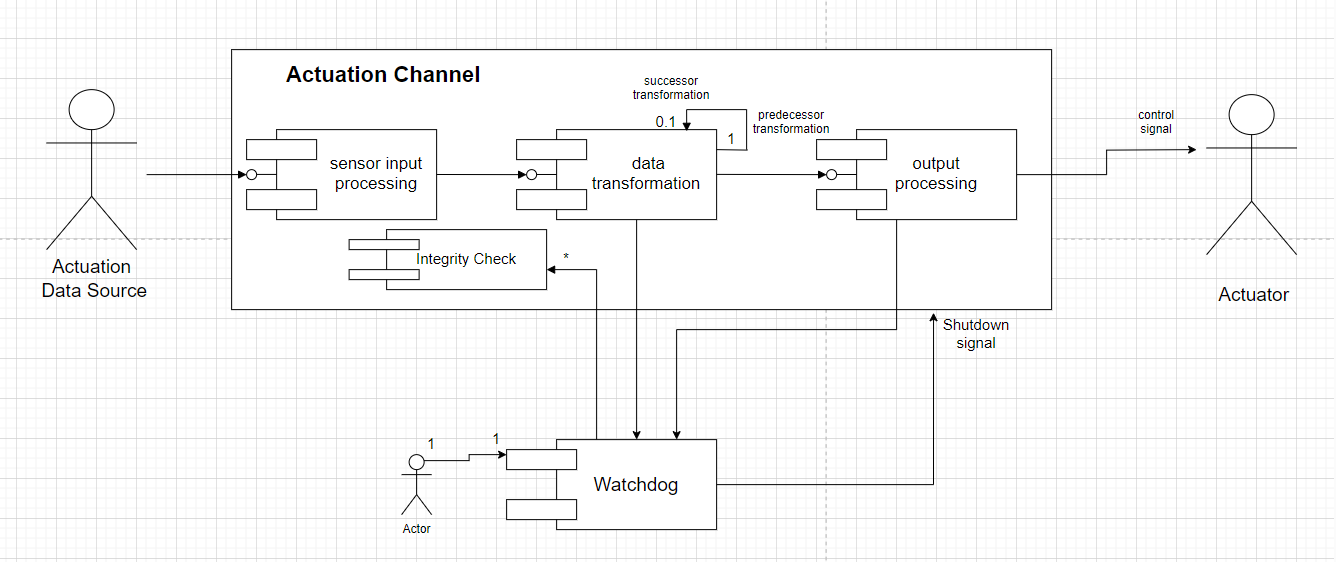
\includegraphics[scale=0.5]{images/third/watchdog.png}
\caption{ساختار الگوی \lr{Watchdog}}
\end{figure}
\subsubsection{الگوی \lr{Safety Executive}}
\label{archSafeSafetyExecSec}
\begin{RTL}
این الگو \cite{ref4}
برای سیستم‌هایی طراحی شده است که اقدامات ایمنی پیچیده‌ای دارند
و نمی‌توان آنها را به سادگی با خاموش کردن سیستم به دست آورد.
این الگو یک جزء مجری ایمنی معرفی می‌کند تا چندین کانال
و اقدامات ایمنی را مدیریت و هماهنگ کند و سیستم را از طریق
یک سری مراحل به وضعیت ایمن هدایت کند. این الگو به‌ویژه برای سیستم‌هایی
که با مواد خطرناک یا حالت‌های پرانرژی کار می‌کنند و خاموشی فوری می‌تواند
خطرناک باشد، مفید است. پیاده‌سازی این الگو پیچیده است و معمولاً
برای سیستم‌های بسیار حساس به ایمنی استفاده می‌شود و در
چنین محیط‌هایی حفاظت عالی در برابر خطا ارائه می‌دهد.
\end{RTL}
\begin{figure}[h!]
\centering
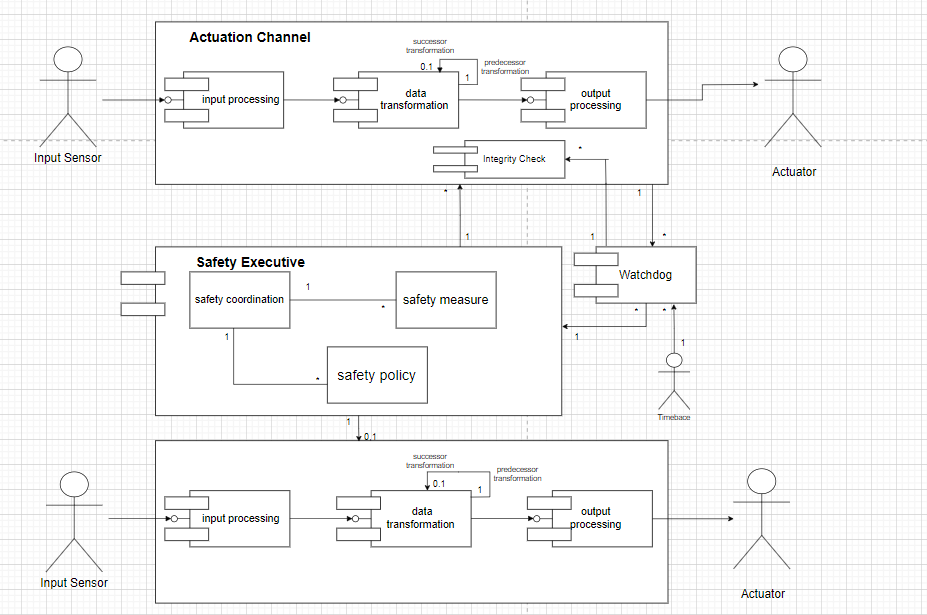
\includegraphics[scale=0.5]{images/third/safetyExec.png}
\caption{ساختار الگوی \lr{Safety Executive}}
\end{figure}